\documentclass[twoside,twocolumn]{article}

\usepackage{blindtext} % Package to generate dummy text throughout this template 
\usepackage{graphicx}
\usepackage[sc]{mathpazo} % Use the Palatino font
\usepackage[T1]{fontenc} % Use 8-bit encoding that has 256 glyphs
\linespread{1.05} % Line spacing - Palatino needs more space between lines
\usepackage{microtype} % Slightly tweak font spacing for aesthetics

\usepackage[english]{babel} % Language hyphenation and typographical rules

\usepackage[hmarginratio=1:1,top=32mm,columnsep=20pt]{geometry} % Document margins
\usepackage[hang, small,labelfont=bf,up,textfont=it,up]{caption} % Custom captions under/above floats in tables or figures
\usepackage{booktabs} % Horizontal rules in tables

\usepackage{lettrine} % The lettrine is the first enlarged letter at the beginning of the text

\usepackage{enumitem} % Customized lists
\setlist[itemize]{noitemsep} % Make itemize lists more compact

\usepackage{abstract} % Allows abstract customization
\renewcommand{\abstractnamefont}{\normalfont\bfseries} % Set the "Abstract" text to bold
\renewcommand{\abstracttextfont}{\normalfont\small\itshape} % Set the abstract itself to small italic text

\usepackage{titlesec} % Allows customization of titles
\renewcommand\thesection{\Roman{section}} % Roman numerals for the sections
\renewcommand\thesubsection{\roman{subsection}} % roman numerals for subsections
\titleformat{\section}[block]{\large\scshape\centering}{\thesection.}{1em}{} % Change the look of the section titles
\titleformat{\subsection}[block]{\large}{\thesubsection.}{1em}{} % Change the look of the section titles

\usepackage{fancyhdr} % Headers and footers
\pagestyle{fancy} % All pages have headers and footers
\fancyhead{} % Blank out the default header
\fancyfoot{} % Blank out the default footer
\fancyhead[C]{Estructuras de Datos y Base de Datos relacionales $\bullet$ Octubre 2020 $\bullet$ } % Custom header text
\fancyfoot[RO,LE]{\thepage} % Custom footer text

\usepackage{titling} % Customizing the title section

\usepackage{hyperref} % For hyperlinks in the PDF

%----------------------------------------------------------------------------------------
%	TITLE SECTION
%----------------------------------------------------------------------------------------

\setlength{\droptitle}{-4\baselineskip} % Move the title up

\pretitle{\begin{center}\Huge\bfseries} % Article title formatting
\posttitle{\end{center}} % Article title closing formatting
\title{Estructuras de Datos y Base de Datos relacionales} % Article title
\author{Arias, Cancino, Crispin, Gutierrez, Zuñiga} 
\date{\today} % Leave empty to omit a date
\renewcommand{\maketitlehookd}{%
\begin{abstract}
	\begin{center}
		\textbf{Resumen}
	\end{center}
	En la era actual, todas las personas están conectadas directa o indirectamente con los conceptos de estructuras de datos y bases de datos y consideran que ambos conceptos son diferentes. Pero la realidad es que la base de datos y la estructura de datos tienen alguna relación entre ellas.
Sin duda, la base de datos es una colección de datos que se pueden almacenar, actualizar y recuperar en cualquier momento cuando sea necesario. Pero cuando se trata de almacenar datos en una base de datos, muchas decisiones sobre cómo se almacenarán los datos. ¿Con qué eficiencia se pueden recuperar los datos de la base de datos? Cuán eficientemente se pueden modificar los datos en la base de datos y surgen muchas preguntas.
Una de las soluciones para tal problema es usar los conceptos de estructuras de datos que pueden involucrar la forma en que se almacenarán los datos, una recuperación fácil y eficiente, etc.
La estructura de datos se refiere a la implementación real del tipo de datos y ofrece una forma de almacenar datos de manera eficiente. La estructura de datos es el resultado de la aplicación de ciertas herramientas y técnicas utilizadas para conectar elementos de datos dentro de registros y entre registros del mismo archivo o de diferentes archivos. Una selección y un diseño adecuados de la estructura de datos ayuda a los usuarios a acceder y manipular los registros de archivos en una base de datos de manera eficiente. El objetivo principal de una estructura de datos es organizar los datos para que se adapten a un propósito específico, de modo que se pueda acceder a los datos y trabajar de manera eficiente y efectiva. La estructura de datos puede diseñarse para almacenar datos con el fin de trabajar en ellos mediante el uso de diferentes algoritmos para buscar o clasificar datos. Los algoritmos son el aspecto esencial de las estructuras de datos y, como existen muchos algoritmos para buscar y clasificar, difieren en términos de eficiencia. Cuando se trata de eficiencia, sería bueno tener métricas para comparar la eficiencia del algoritmo.
\\
	\begin{center}
		
		\textbf{Abstract}
	\end{center}
	In today's age, all people are directly or indirectly connected with the concepts of data structures and databases and consider that both concepts are different. But the reality is that the database and the data structure have some relationship between them. 
Without doubt, the database is a collection of data that can be stored, updated, and retrieved at any time when needed. But when it comes to storing data in a database, many decisions about how the data will be stored. How efficiently can the data be retrieved from the database? How efficiently can the data in the database be modified and many questions arise. 
One of the solutions for such a problem is to use the concepts of data structures that may involve the way the data will be stored, easy and efficient retrieval, etc. 
The data structure refers to the actual implementation of the data type and offers a way to store data efficiently. The data structure is the result of the application of certain tools and techniques used to connect data elements within records and between records in the same file or in different files. Proper selection and design of the data structure helps users to access and manipulate the file records in a database efficiently. The main goal of a data structure is to organize the data to suit a specific purpose, so that the data can be accessed and worked efficiently and effectively. The data structure can be designed to store data in order to work on it by using different algorithms to find or classify data. Algorithms are the essential aspect of data structures, and since there are many algorithms to search and classify, they differ in terms of efficiency. When it comes to efficiency, it would be nice to have metrics to compare the efficiency of the algorithm.
	\\
\end{abstract}
}

%----------------------------------------------------------------------------------------

\begin{document}

% Print the title
\maketitle

%----------------------------------------------------------------------------------------
%	ARTICLE CONTENTS
%----------------------------------------------------------------------------------------

\section{Introduccion}

\lettrine[nindent=0em,lines=3]{O}rganizar la información en función de una rápida recuperación es indudablemente un factor determinante en muchos sectores de la actividad sin olvidar las necesidades tanto en el ámbito de decisión, como el consultar y analizar siempre meas cantidad de información; hasta, por ejemplo, con pensar en el problema cotidiano del que administra un almacén o una biblioteca. De ahí la utilidad de organizar la información en estructuras fácilmente administrables y que aseguren una elevada velocidad de acceso.
Existen factores muy interesantes en la fase de proyectar y realizar una base de datos, factores de notable interés conceptual sobre todo si se ve la planificación de la base de datos con el momento de ordenación y construcción de la realidad en términos de entidad y de su interrelación.



%------------------------------------------------
%-----------------------------------------------------------------
\section {Desarrollo}\label{sec:3}
\subsection{ESTRUCTURA DE DATOS}
Estas son las que nos permiten almacenar, manipular y ordenar datos los cuales son materia prima en todo tipo de información.
diferentes tipos de estructura de datos y estas son adecuadas para diferentes tipos de aplicaciones y algunas de estas son especializados en tipos de áreas específicas. Con las estructuras de datos también se pueden manejar grandes cantidades de datos de manera eficiente para usos tales como grandes bases de datos de la Internet . Las estructuras de datos son excelentes más que todo para diseñar algoritmos eficientes.

\begin{itemize}
	\item \textbf{OPERACIONES BASICAS EN UNA ESTRUCTURA DE DATOS}
	\\
	\\Las estructuras de datos nos permiten operaciones simples que nos dejan manipular cualquier tipo de información y entre estas tenemos:
	\begin{itemize}
		\item Adicionar
		\item Búsqueda
		\item Recorrer
		\item Eliminar
		
	\end{itemize}
	
	\item \textbf{IMPORTANCIA DE LA ESTRUCTURA DE DATOS}
	\\
	\\Lo que caracteriza y hace importante a lo que llamamos estructura de datos principal mente es su eficiencia su riqueza para el procesamiento de datos y sus estructuras simples. Las estructuras de datos simples se pueden combinar de distintas formas más estructuradas y complejas.
	\\
	\item \textbf{CAMPOS IMPORTANTES}
	
	\begin{itemize}
		\item \textbf{PRIMITIVAS:} Son aquellas que no están compuestas por otra estructura de datos como, por ejemplo:
        \begin{itemize}
            \item Char
            \item Double
            \item Int
            \item Boolean
        \end{itemize}
        \item \textbf{NO PRIMITIVAS:} Son aquellas que están compuestas en su estructura entre estas tenemos
        \begin{itemize}
            \item Lineales
            \item No lineales
        \end{itemize}
    \end{itemize}
    
	\item \textbf{TIPOS DE ESTRUCTURAS}
	\\
	\\Estos patrones de diseño tienen que ver con la comunicación de objetos de Class. Los patrones de comportamiento son aquellos que se ocupan más específicamente de la comunicación entre objetos.
	\begin{itemize}
		\item \textbf{ESTRUCTURAS LINEALES:} \\Estas se caracteriza por poseer el principio de adyacente es decir están almacenados contiguamente entre estas están
        \begin{itemize}
            \item \textbf{Pilas:} Estructura de datos lineales donde los elementos pueden ser añadidos o removidos solo por un extremo. Estas trabajan con filosofía LIFO (LAST IN-FIRST OUT).
            \begin{center}
                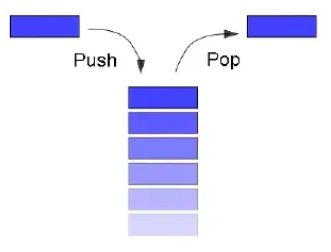
\includegraphics[width=5cm]{./img/1.png} 
            \end{center}
            \item \textbf{Colas:} Es una estructura de datos se caracteriza por ser una secuencia de elementos en la que la operación de inserción push se realiza por un extremo y la operación de extracción pop por el otro también se llama estructura FIFO (FIRST IN-FIRST OUT).
            \begin{center}
                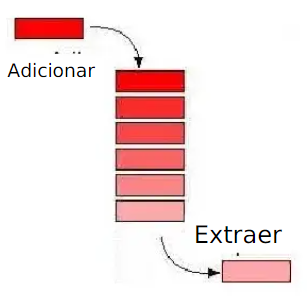
\includegraphics[width=5cm]{./img/2.png} 
            \end{center}
            \item \textbf{Listas enlazadas:} Es aquella que permite almacenar datos de una forma organizada, al igual que los vectores, pero, a diferencia de estos, esta estructura es dinámica, por lo que no tenemos que saber os elementos que puede contener. En una lista enlazada, cada elemento apunta al siguiente excepto el último que no tiene sucesor y el valor del enlace . Por ello los elementos son registros que contienen el dato a almacenar y un enlace al siguiente elemento. Los elementos de una lista suelen recibir también el nombre de nodos de la lista.
            \begin{center}
                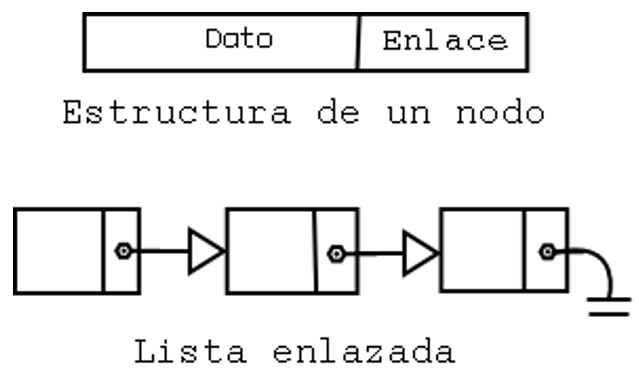
\includegraphics[width=5cm]{./img/3.png} 
            \end{center}
        \end{itemize}
        \item \textbf{ESTRUCTURAS NO LINEALES: }\\ Son aquellas que no posee principio ni adyacente es decir no están contiguamente entre ellas están:
		\begin{itemize}
            \item \textbf{Arboles:} Son las estructuras de datos más utilizadas, pero también una de las más complejas, Los Árboles se caracterizan por almacenar sus nodos en forma jerárquica y no en forma lineal como las Listas, Colas, Pilas, etc.
            \begin{center}
                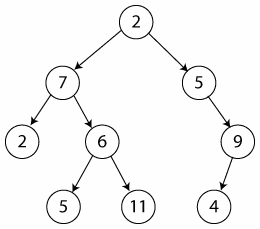
\includegraphics[width=5cm]{./img/4.png} 
            \end{center}
            \item \textbf{Grafos:} Consiste en un conjunto de nodos y un conjunto de arcos que establecen relaciones entre los nodos.
            \begin{center}
                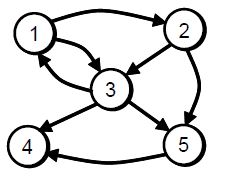
\includegraphics[width=5cm]{./img/5.png} 
            \end{center}
        \end{itemize}
	\end{itemize}
\end{itemize}

\subsection{ESTRUCTURA DE BASE DE DATOS RELACIONALES}
Hay cosas en un entorno empresarial sobre las que necesitamos almacenar datos, y esas cosas están relacionadas entre sí de diversas formas. De hecho, para ser considerado una base de datos, el lugar donde se almacenan los datos debe contener no solo los datos sino también información sobre las relaciones entre esos datos. Por ejemplo, podríamos necesitar relacionar a nuestros clientes con los pedidos que nos hacen y los artículos de nuestro inventario con los pedidos de esos artículos.
La idea detrás de una base de datos es que el usuario, ya sea una persona que trabaja de forma interactiva o un programa de aplicación, no tiene que preocuparse por cómo se almacenan físicamente los datos en el disco. El usuario formula solicitudes de manipulación de datos en términos de relaciones de datos. Un software conocido como sistema de gestión de bases de datos (DBMS) se traduce luego entre la solicitud de datos del usuario y el almacenamiento de datos físicos.
Entonces, ¿por qu
é los simples paquetes de software de bases de datos (los administradores de listas) no producen verdaderas bases de datos? Debido a que no pueden representar relaciones entre datos, mucho menos usan tales relaciones para recuperar datos. El problema es que el software de gestión de listas se ha comercializado durante años como base de datossoftware, y muchos compradores no comprenden exactamente lo que están comprando. Lo que empeora el problema es que un área rectangular de una hoja de cálculo también se llama base de datos . Como verá más adelante en este libro, un grupo de celdas en una hoja de cálculo es incluso menos una base de datos que una lista independiente. Debido a que persiste este problema de terminología, también permanece la confusión acerca de qué es exactamente una base de datos.
\begin{itemize}
	\item \textbf{TABLES}
	\\
	\\Una base de datos relacional es una colección de tablas de datos relacionados. Las columnas describen la información específica en la tabla y cada fila almacena los datos correspondientes.
    Por ejemplo, una tabla "Cliente" puede contener columnas:
    \\
    \begin{center}
        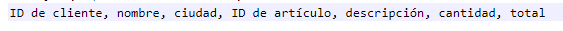
\includegraphics[width=5cm]{./img/6.png} 
    \end{center}
    
    La tabla tendría entonces los datos del cliente almacenados en las filas de la tabla.
	\\
	\item \textbf{PRIMARY KEYS}
	\\
	\\Una clave principal es una columna o compilación de varias columnas que tiene un valor único, lo que hace que cada fila sea única en la tabla.
    Cada tabla debe tener una clave principal porque se usa para vincular datos en tablas relacionadas . Por ejemplo, la clave principal de la tabla Cliente sería la columna denominada "CustomerId", mientras que la tabla Historial de pedidos puede tener "OrderID" como clave principal.
    \\
	\item \textbf{FOREIGN KEYS}
	\\
	\\Una clave externa es la clave principal de otra tabla y se usa para relacionar filas de datos entre tablas.
    Por ejemplo, la tabla Historial de pedidos tiene una clave principal de "OrderId" para identificar cada registro. Para saber qué cliente realizó el pedido, los datos de la columna "CustomerID" del cliente de la tabla Cliente se almacenan en la fila Historial de pedidos. Luego, se pueden realizar consultas para unir los datos de ambas tablas en aplicaciones comerciales.
    
\end{itemize}
\subsection{BENEFICIOS}
\begin{itemize}
	\item Permite un procesamiento de datos más sencillo.
	\item Permite almacenar información en disco de manera muy eficiente.
	\item Estos son necesarios para diseñar un algoritmo eficiente.
	\item Proporciona administración de bases de datos como indexación con la ayuda de tablas y matrices hash.
	\item Podemos acceder a los datos en cualquier momento y en cualquier lugar.
	\item Es una forma segura de almacenamiento de datos.
	\item Modelos de gráficos problemas de la vida real 
	\item Permite el procesamiento de datos en el sistema de software.
\end{itemize}

\subsection{PERJUICIOS}

\begin{itemize}	
\item Es aplicable solo para usuarios avanzados.
\item Si surge algún problema, solo los expertos pueden resolverlo.
\item Acceso lento en caso de algunos tipos de datos.
\end{itemize}
\section{Ejemplo Pilas}

\begin{center}
	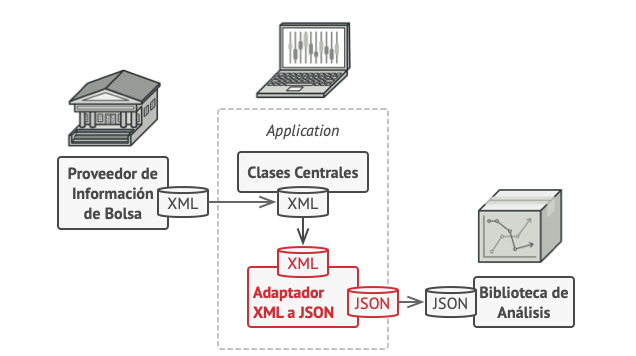
\includegraphics[width=5cm]{./img/7.png} 
\end{center}

\begin{center}
	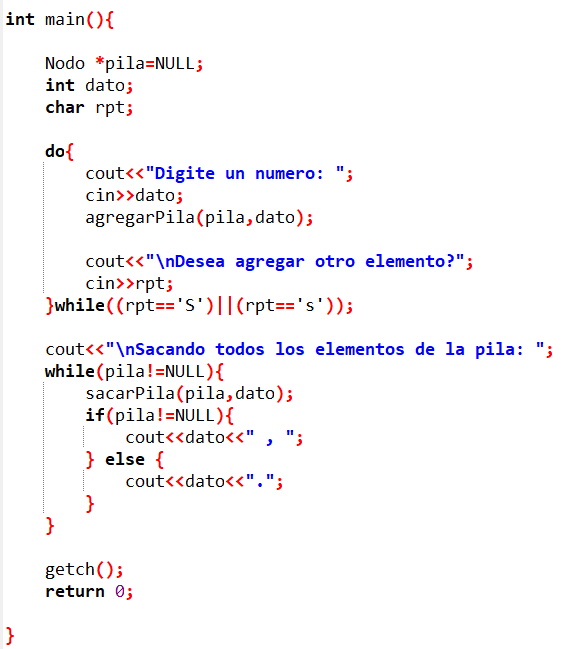
\includegraphics[width=5cm]{./img/8.png} 
\end{center}

\begin{center}
	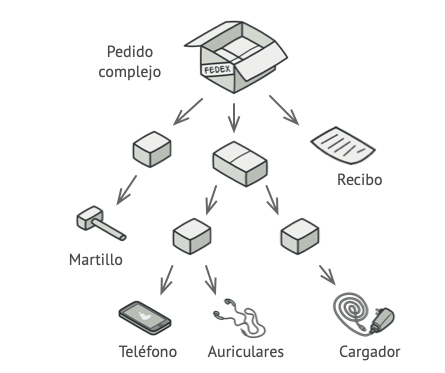
\includegraphics[width=5cm]{./img/9.png} 
\end{center}

\section{Conclusiones}


Mediante el desarrollo de este trabajo se ha logrado desarrollar y entender el curso de Estructura de Datos.

Conocedores que su realización nos han permitido el aprendizaje en los diferentes temas y están contribuyendo al cambio de nuestra manera de vivir, con ello nuestra formación profesional.

La conclusión a lo que se ha llegado con el desarrollo de este importante curso en nuestra carrera, es a poder estructurar un programa, lo que posteriormente nos facilitará el trabajo en los cursos venideros; utilizando para esto la lógica computacional y la estructuración; llegando a lograr comprender de esta manera que existen muchas soluciones a los problemas planteados tanto aplicados a ejemplos como a la vida real.
\section{Recomendaciones}

Al terminar de definir la estructura de una base de datos, es bueno hacer varios ejercicios llenándola con información real o ficticia para encontrar posibles vacíos, fallas, etc., en el diseño. 

%------------------------------------------------
%-----------------------------------------------------------------

\section{Bibliografia}\label{sec:7}
\begin{itemize}
\item [1] Dina, P. (2015). Estructuras Pi\\las y Colas TDA. Recuperado de https://www.academia.edu/22313790/Pi\\las\_\\y\_Colas \\
\item [2] Blancante, O. (2014). Estructura de datos – Árboles. Recuperado de https://www.oscarblancarteblog.com/201\\4/08/22/estructura-de-datos-arboles/\\
\item [3] Castro, K. (2016). ESTRUCTURA DE UNA BASE DE DATOS. Recuperado de http://castrokatia123.blogspot.com/2016/\\08/estructura-de-base-de-datos.html\\
\item [4] Goyal, N. (2015). IT Article -- DBMS \& Data Structure. Recuperado de http://srimca.edu.in/SRIJAN/Srijanoct20\\08/Articles/IT/DBMS-DS.html\\
\item [5] Hammer, J., \& Schneider, M. (2001). Data Structures for Databases 60.1. Recuperado de: https://www.cise.ufl.edu/\~mschneid/Rese\\arch/papers/HS05BoCh.pdf\\
\item [6] Goodrich, M.T. and Tamassia, R., Data Structures and Algorithms in Java, 6 th Edition, John Wiley, 2014.\\
\item [7] A Silberschatz, H.F. Korth, S. Sudarshan. Database System Concepts 6th Edition. McGraw Hill, 2011\\
\item [8] Hector Garcia-Molina, Jeffrey D. Ullman \& Jennifer Widom. Database System Implementation, Prentice Hall, 3rd Edition, 2008.\\
\end{itemize}
\bibliographystyle{plain}
\bibliography{bibliografia}
\end{document}